\documentclass[final]{elsarticle} %times

\usepackage[colorlinks]{hyperref}

%% Stylefile to load JCOMP template
\usepackage{jcomp}
\usepackage{framed,multirow}

% \usepackage[utf8]{inputenc}
% \usepackage[english]{babel}
% \usepackage[T1]{fontenc}
% \usepackage{csquotes}

%%% Functional packages
\usepackage[tbtags]{amsmath}
\usepackage{amssymb, amsthm}
\usepackage{physics, siunitx}
\usepackage{isomath}        % for \vectorsym, \tensorsym, ...
\usepackage{mathrsfs}       % for \mathscr
\usepackage{mathtools}      % for `multlined` environment
\usepackage{subcaption}     % for `subfigure` environment
\usepackage{suffix}         % for \WithSuffix
\usepackage[referable]{threeparttablex} % for \tnotex
\usepackage{chemformula}    % for \ch
\usepackage{multirow}
\usepackage{xspace}
\usepackage{comment}
\usepackage{graphicx}
    \graphicspath{{_pics/}}
\usepackage{algorithm}
\usepackage[noend]{algpseudocode}  % load `algoritmicx` package as well
    \algnewcommand{\TRUE}{\textbf{true}}
    \algnewcommand{\FALSE}{\textbf{false}}
    \algnewcommand{\OR}{\textbf{ or }}
    \algnewcommand{\AND}{\textbf{ and }}
    \algnewcommand{\VAR}{\texttt}
\usepackage[subfolder]{gnuplottex}

%%% Configuration packages
\usepackage{enumitem}       % for configuration of enumerates

%%% TikZ
\usepackage{tikz}
\usetikzlibrary{shapes, arrows, arrows.meta, chains, positioning, decorations.pathmorphing,
    decorations.pathreplacing, matrix, patterns}

%%% Counter for ray-tracing algorithm
\newcounter{RayTracing}
\newcommand{\RTcase}{\Comment{\refstepcounter{RayTracing}Case \theRayTracing}}

%%% General aliases
\newcommand{\tran}{\mathsf{T}} %{^{\mkern-1.5mu\mathsf{T}}}
\DeclareSIUnit{\wtpercent}{wt\%}
\DeclareMathOperator{\Heaviside}{H}
\newcommand{\mysi}[1]{\si[per-mode=reciprocal]{#1}}

%%% \myoverbrace command (requires `xparse` package)
\NewDocumentCommand{\myoverbracetext}{m}{\text{#1}\\} % for internal use
\NewDocumentCommand\myoverbrace{ O{\int} m >{\SplitList{\\}}m }
{% two mandatory arguments: 2 - formula and 3 - caption delimited by \\
    \overbrace{\vphantom{#1}#2}^{\substack{\ProcessList{#3}{\myoverbracetext}}}
}

%%% Material derivative (requires `suffix` package)
\newcommand\Dv[2][]{\frac{\mathrm{D}#1}{\mathrm{D}#2}}
\WithSuffix\newcommand\Dv*[2][]{\mathrm{D}#1/\mathrm{D}#2}

%%% Problem-specific aliases
\newcommand{\fusion}[1]{{#1}_\text{fus}}
\newcommand{\evapor}[1]{{#1}_\text{vap}}
\newcommand{\gradf}[1]{\grad_{\!\! #1}}
\newcommand{\OpenFOAM}{OpenFOAM\textregistered\xspace}
\newcommand{\Cp}[1]{\mathfrak{c}_{p#1}}
\newcommand{\SourceTerm}{\mathscr{F}}
\newcommand{\Abso}{\mathcal{A}}
\newcommand{\Refl}{\mathcal{R}}
\newcommand{\sol}{\text{S}}
\newcommand{\liq}{\text{L}}
\newcommand{\gas}{\text{G}}
\newcommand{\boil}{\text{b}}
\newcommand{\melt}{\text{m}}
\newcommand{\laser}{\ell} % \text{l}
\newcommand{\viewfactor}[3]{{#1}_{\dd{S}#2\to\dd{S}#3}}
\newcommand{\dviewfactor}[4][]{{\dv{\viewfactor{#2}{#3}{#4}#1}{S#4}}}

%%% Bold symbols
\newcommand{\bv}{\vb*{v}}
\newcommand{\bn}{\vu*{n}}
\newcommand{\bs}{\vu*{s}}
\newcommand{\bi}{\vu*{\imath}}
\newcommand{\br}{\vu*{r}}
\newcommand{\bt}{\vu*{t}}
\newcommand{\bx}{\vb*{x}}
\newcommand{\bg}{\vb*{g}}
\newcommand{\bp}{\vb*{p}}
\newcommand{\btau}{\tensorsym{\tau}}
\newcommand{\bI}{\matrixsym{I}}

%%% For algorithms
\newcommand{\V}{V}
\newcommand{\dV}{\partial V}
\newcommand{\intCell}{\int_{\V}}
\newcommand{\intFaces}{\oint_{\dV}\!\!\!\bn}
\newcommand{\implicit}[1]{\underbrace{#1}_\text{implicit}}
\newcommand{\explicit}[1]{\underbrace{#1}_\text{explicit}}
\newcommand{\linearization}[1]{\underbrace{#1}_\text{linearization}}

%%% Dimensionless numbers
\newcommand{\Mach}{\operatorname{\mathit{M\kern-.10em a}}}
\newcommand{\Pecl}{\operatorname{\mathit{P\kern-.08em e}}}
\newcommand{\Reyn}{\operatorname{\mathit{R\kern-.04em e}}}

%%% For coloring
\usepackage{xcolor}
%\newcommand{\alert}[1]{\textcolor{red}{\bf #1}}
\newcommand{\alert}[1]{\textcolor{red}{#1}} % for highlighting
\newcommand{\Oleg}[1]{\protect\footnote{\textcolor{magenta}{Oleg: #1}}} % Oleg's remarks
\newcommand{\ak}[1]{\protect\footnote{\textcolor{blue}{Aslan: #1}}} % Aslan's remarks

\journal{Journal of Computational Physics}

\begin{document}

\begin{frontmatter}

\title{High-fidelity simulation of the keyhole dynamics\tnoteref{tnote1}}
\tnotetext[tnote1]{Just a first attempt.}
\author[1]{Oleg A. \snm{Rogozin}\corref{cor1}}
\ead{o.rogozin@skoltech.ru}
\author[1]{Aslan R. \snm{Kasimov}}
\ead{a.kasimov@skoltech.ru}
\address[1]{\alert{Center of Materials \& Technologies},
    Skolkovo Institute of Science and Technology,
    Bolshoy Boulevard 30, bld. 1, Moscow, 121205, Russia}

\begin{abstract}
%%% Aim
In this work, we investigate numerically the melt-pool dynamics including the keyhole formation.
The governing system of three-dimensional three-phase fluid dynamics equations
includes a wide range of physical effects such as: surface-tension with Marangoni stresses,
evaporation of the melt, solidification, and temperature dependence of various fluid properties.
%
%%% Assumptions
All three phases are modeled as incompressible viscous heat-conducting fluids.
The solidification of the melt is assumed to take place over a homogenized mushy layer
modeled as a porous medium.
%
%%% Implementation and validation
The proposed thermo-fluid-dynamic model is implemented in the \OpenFOAM environment
and is validated against experimental data.
Excellent agreement is found with respect to the form and dimensions of the solidified track.
The role of various physical effects that are included in the model is analyzed
and their importance is discussed.
\end{abstract}

\end{frontmatter}

\tableofcontents

\section{Introduction}

% [Oleg] This paragraph is taken from Oerlikon report
Fluid-dynamics of the melt pool is the crucial physical process
for predicting the resulting properties of a printed part.
In turn, this affects the uniformity of the printing and, very likely, the details of the grain formation
and the residual stresses in the printed part.
Furthermore, the melt-pool dynamics is expected to strongly influence the solidification-front evolution
and structure via local temperature gradients, which are coupled to the fluid flow.
A detailed exploration of these processes is a significant challenge for modeling
that should be undertaken in a follow-up work.

\section{Mathematical model}\label{sec:model}

The present mathematical model has been developed based on and influenced by a number of
published works, such as~\cite{cho2006implementation, attar2011simulation, qiu2015role, khairallah2016laser,
wang2019powder, cook2019simulation, khairallah2020controlling}.
Much physics is unified in order to formulate a single multi-physics system of governing equations
that is capable of treating different phase states and their inter-phase conditions
within a single system of fluid-dynamic equations.
The laser radiation is considered as a collimated beam with a pure specular reflection on gas--metal interface.

\subsection{Assumptions}

%%% Assumptions of the model
The physical model employed in our study is subject to the following assumptions:
\begin{itemize}
    \item Gas, liquid, and solid are incompressible fluids with constant densities.
    \item Laser radiation is absorbed uniformly over the surface with a constant absorptivity, regardless of the angle of incidence.
    \item Solid media are at rest.
    \item The liquid behaviour is Newtonian with Arrhenius temperature dependence.
    \item The solidification interface is modeled as a mushy layer.
\end{itemize}
The last assumption allows us to model the solidification front structure as a porous medium
with a given permeability and to avoid computing the multi-scale complex structure
of the solidification front dynamics at the present level of modeling.
The following physical phenomena are described by the model:
\begin{itemize}
    \item Surface tension and thermal Marangoni effect.
    \item Solidification and evaporation of the molten metal.
    \item Recoil pressure and evaporative cooling (very important to suppress superheating).
    \item Radiative (thermal and laser) and convective heat transfer.
    \item The fluid flow in melt pool is Newtonian and laminar~\cite{tang2018numerical}.
    \item The thermophysical properties of SS316L are functions of temperature only~\cite{tang2018numerical}.
\end{itemize}
Moreover, the following physical effects are neglected:
\begin{itemize}
    \item Plasma effect in the SLM process is ignored~\cite{tang2018numerical}.
    \item Viscous heat dissipation.\Oleg{I have already included it in code.}
    \item Wetting force.
    \item Chemical Marangoni effect.
    \item Optics, including absorption of the reflected laser radiation, shadow effects, and beam divergence.
    \item Shrinkage due to the density change as a function of temperature and phase transition.
    \item Kinetic energy of fluid flow.
    \item Vapor mass losses.
    \item Mechanical stresses in solid body.
    \item Difference between solidus and liquidus.
\end{itemize}
Finally, some minor assumptions:
\begin{itemize}
    \item The laser beam has a Gaussian spatial distribution.
    \item Heat capacity and thermal conductivity are linear functions of temperature~\cite{le2019study}.
    \item The densities of liquid and solid metal are equal to each other.
    \item Viscosity of the gas does not depend on temperature.
    \item Viscosity of the metal obeys Andrade equation~\cite{andrade1930viscosity}.
    \item Enthalpy of evaporation does not depend on temperature.
\end{itemize}

\subsection{Governing equations}

%%% On three phases
The model is based on equations of fluid mechanics for three phase states,
which are identified by the following variables: $\alpha\in\{0,1\}$ is the metal fraction,
$\phi$ is the volume fraction of the molten metal.
Then, all pure-phase states are identified as follows:
\begin{enumerate}[label=\arabic*)]
    \item gas: $\alpha=0$, $\phi=0$;
    \item liquid: $\alpha=1$, $\phi=1$;
    \item solid: $\alpha=1$, $\phi=0$.
\end{enumerate}
The solid--liquid interface is smoothed out via continuous change of $\phi$ over the mushy layer.
In the present formulation, the solid phase is stationary, i.e., $\bv=0$,
and is obtained from the fluid state in the limit $\phi\to0$.
Thus, the detailed modeling of the solid-phase structure is beyond the scope of the present model,
which focuses on the phase transition between the solid and liquid states including heat transfer processes.

%%% Governing equations
The governing equations for density $\rho$, velocity $\bv$, pressure $p$, and specific enthalpy $h$ are as follows:
\begin{gather}
    \pdv{\alpha}{t} + \bv\vdot\grad\alpha = 0, \label{eq:alpha}\\
    \div\bv = 0, \label{eq:continuity}\\
    \begin{multlined}
    \rho\qty(\pdv{\bv}{t} + \bv\vdot\grad\bv) =
        - \myoverbrace{K\alpha\qty(\frac{\alpha-\phi}{\phi})^2\bv}{Darcy force}
        + \myoverbrace{\div\btau}{viscous\\force}
        - \myoverbrace{\grad{p}}{pressure\\force}
        + \myoverbrace{\rho\bg}{gravity\\force}
        - \myoverbrace{\rho\bg\beta(T-T_0)}{buoyancy force}\\
        - \myoverbrace{\gamma\qty(\div\bn_\alpha)\gradf{\rho}\alpha}{surface tension}
        + \myoverbrace{\dv{\gamma}{T}\qty(\bn_\alpha\cp\grad{T}\cp\bn_\alpha)
            |\gradf{\rho}\alpha|}{Marangoni force}
        - \myoverbrace{\frac{3-\evapor{a}}4\evapor{p}\gradf{\rho}\alpha}{recoil pressure},
    \end{multlined}\label{eq:v}\\
    \begin{multlined}
    \rho\qty(\pdv{h}{t} + \bv\vdot\grad h)
        = \myoverbrace[\qty(\frac12)^2]{\div(k\grad{T})}{heat conduction}
        + \myoverbrace{\int_{\partial\Omega_\gas}\!\!\! I_\laser(\bx')
            \dviewfactor[(\bs_\laser)]{\mathscr{F}}{'}{} \dd{S}'
            |\gradf{\rho c_p}\alpha|}{laser heat source}\\
        - \myoverbrace{\epsilon\sigma\qty(T^4-T_0^4)|\gradf{\rho c_p}\alpha|}{radiative cooling}
        - \myoverbrace{\frac{\evapor{a}\evapor{p}\evapor{h}}
            {(2\pi RT/M_\liq)^{1/2}}|\gradf{\rho c_p}\alpha|}{evaporative cooling},
    \end{multlined}\label{eq:h}
\end{gather}
where $K>0$ is the coefficient related to the permeability of the mushy layer,
$\bg$ is the gravitational acceleration,
$\beta$ is the volumetric thermal expansion coefficient,
$T_0$ is the ambient temperature,
$\gamma$ is the surface tension,
$\bn_\alpha \equiv \grad\alpha/|\grad\alpha|$ is the unit vector
normal to the gas--metal interface and pointing into the metal,
$k$ is the thermal conductivity,
$\partial\Omega_\gas$ is the part of the boundary where $\alpha = 0$,
$\dd{S}$ is the infinitesimal area of the gas--metal interface,
$\bs_\laser$ is the unit vector in the direction of the laser beam,
$\epsilon$ is the emissivity of the metal surface,
$\sigma$ is the Stefan--Boltzmann constant,
$0 < \evapor{a} < 1$ is the evaporation coefficient,
$\evapor{h}$ is the enthalpy of vaporization,
$M_\liq$ is the molar mass of the alloy,
$R$ is the universal gas constant.

%%% Other quantities
Temperature $T$, viscous stress tensor $\btau$, vapor pressure $\evapor{p}$, liquid fraction $\phi$,
laser beam intensity $I_\laser$, modified gradient $\gradf{f}$,
and radiation exchange factor $\dd\viewfactor{\mathscr{F}}{'}{}$ between surface elements $\dd{S'}$ and $\dd{S}$
are calculated from the following relations:
\begin{gather}
    h = \int_0^T c_p(\alpha,\xi)\dd{\xi} + \fusion{h}\phi(\alpha,h), \label{eq:T}\\
    \btau = \mu\qty(\grad\bv + \qty(\grad\bv)^\tran), \label{eq:tau}\\
    \evapor{p}(T) = p_0\exp(\frac{M_\liq\evapor{h}}{R}\qty(\frac1{T_\boil}-\frac1{T})),
        \label{eq:p_evapor}\\
    \phi(\alpha,h) = \alpha\mathcal{S}\qty(\frac{h-h_\melt(\alpha)}{\fusion{h}}),
        \label{eq:phi}\\
    h_\melt(\alpha) = \int_0^{T_\melt} \!\! c_p(\alpha,\xi)\dd{\xi} + \frac{\alpha\fusion{h}}2,
        \label{eq:h_melt}\\
    I_\laser(\bx) = \frac{2P}{\pi R_\laser^2}
        \exp(-2\frac{\qty|(\bx-\bx_\laser)\cp\bs_\laser|^2}{R_\laser^2}), \label{eq:Ilaser}\\
    \gradf{f} = \frac{2f(\alpha)}{f(0)+f(1)}\grad, \label{eq:gradf}\\
    \begin{split}
        \dviewfactor[(\bi)]{\mathscr{F}}{'}{} &= \viewfactor{\Abso}{'}{}\dviewfactor[(\bi)]{F}{'}{} \\
        &+ \int_{|\grad\alpha|\neq0} \!\!\! \dviewfactor[(\bi)]{F}{'}{_*}\qty(1-\viewfactor{\Abso}{'}{_*})
            \dviewfactor[(\br)]{\mathscr{F}}{_*}{}\dd{S}_*,
    \end{split}\label{eq:exchange_factor}\\
    \br = \bi - 2(\bi\vdot\bn_\alpha)\bn_\alpha, \label{eq:reflection}
\end{gather}
where $c_p$ is the heat capacity, $\fusion{h}$ is the enthalpy of fusion,
$\mu$ is the viscosity, $p_0$ is the ambient pressure,
$T_\melt$ and $T_\boil$ are the melting and boiling temperatures, respectively,
$P$ is the laser power, $R_\laser$ is the radius of the laser beam,
$\bx_\laser$ is the intersection point between the laser beam axis and $\partial\Omega_\gas$,
$\viewfactor{\Abso}{_i}{_j}$ is the fraction of laser radiation coming from $\dd{S_i}$
and being absorbed by metal surface element $\dd{S_j}$,
$\bi$ and $\br$ are the direction vectors of the incident and reflected rays, respectively.

%%% View factor
The view factor $\dd\viewfactor{F}{_i}{_j}$ between surface elements $\dd{S_i}$ and $\dd{S_j}$
is a geometric function defined as the fraction of energy leaving $\dd{S_i}$ directly toward
and intercepted by $\dd{S_j}$, where the word ``directly'' means ``on a straight path,
without intervening reflections''~\cite{modest2013radiative}.
In the case of a directional irradiation along $\bs_i$,
\begin{equation}\label{eq:view_factor}
    \dviewfactor[(\bs_i)]{F}{_i}{_j} = \sum_k\delta(\bx_i-\bx_k),
\end{equation}
where $\bx_k$ is an enclosure point for which $(\bx_k-\bx_j)\cp\bs_i = 0$,
and the recurrence formula~\eqref{eq:exchange_factor} is expanded to a sum of two-dimensional
Dirac delta functions as illustrated in Fig.~\ref{fig:exchange_factor}.

\begin{figure}
    \centering
    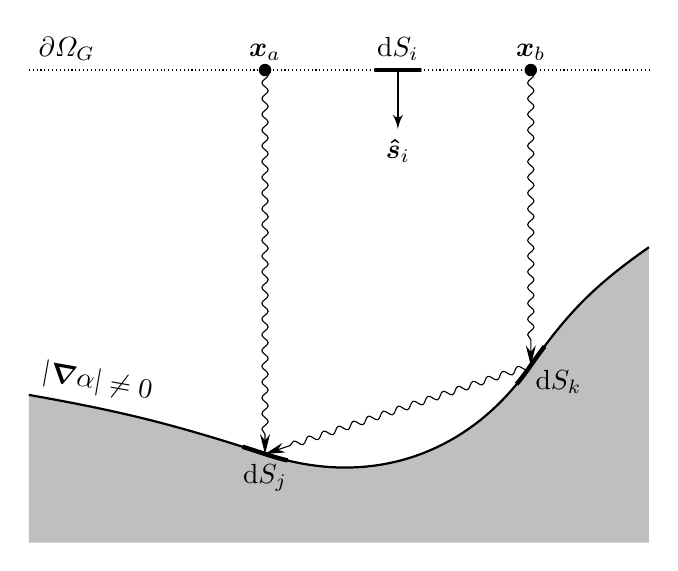
\begin{tikzpicture}[
            metal/.style={fill=gray!50},
            interface/.style={thick},
            dS/.style={ultra thick},
            ray/.style={->, decorate, decoration={snake, amplitude=.4mm, segment length=2mm, post length=2.5mm}},
            vector/.style={->, thick, >=latex'},
            >={Stealth[scale length=1.5]},
            scale=1.5
        ]
        \pgfmathsetmacro{\dSlength}{0.2}

        \coordinate (t1) at (-3.5, 1);
        \coordinate (t2) at (-1.5, 1);
        \coordinate (t3) at (0.75, 1);
        \coordinate (t4) at (1.75, 1);

        \coordinate (b1) at (-3.5, -1.75);
        \coordinate (b2) at (-1.5, -2.25);
        \coordinate (b3) at (0.75, -1.5);
        \coordinate (b4) at (1.75, -0.5);

        \coordinate (c1) at (-3.5, -3);
        \coordinate (c2) at (1.75, -3);

        \draw[densely dotted] (t1) node[above right] {$\partial\Omega_G$} -- (t2)
            to node[above] {$\dd{S_i}$} coordinate (t5) (t3) to (t4);
        \draw[vector] (t5) -- +(0,-.5) node[below] {$\bs_i$};

        \fill[metal] (b1)
            to[bend left=4] (b2)
            to[bend right=37] (b3)
            to[bend left=10] (b4)
            to (c2) -- (c1);

        \draw[interface] (b1)
            to[bend left=4] node[above right, at start, sloped] {$|\grad\alpha|\neq0$} (b2) node[below] {$\dd{S_j}$}
            to[bend right=37] (b3) node[below right=-0.1] {$\dd{S_k}$}
            to[bend left=10] (b4);

        \begin{scope}
            \clip (b2) circle [radius=\dSlength];
            \draw[dS] (b1)
                to[bend left=4] (b2)
                to[bend right=37] (b3);
        \end{scope}

        \begin{scope}
            \clip (b3) circle [radius=\dSlength];
            \draw[dS] (b2)
                to[bend right=37] (b3)
                to[bend left=10] (b4);
        \end{scope}

        \begin{scope}
            \clip (t5) circle [radius=\dSlength];
            \draw[dS] (t2) -- (t3);
        \end{scope}

        \foreach \Point/\Place/\Index in {t2/above/a, t3/above/b}
            \fill (\Point) circle[radius=1.5pt] node[\Place] {$\bx_\Index$};

        \foreach \From/\To in {t2/b2, t3/b3, b3/b2}
            \draw[ray] (\From) to (\To);
    \end{tikzpicture}
    \caption{
        A vertically collimated (along $\bs_i$) laser beam incident on the metal surface.
        The snake arrows represent single rays.
        The radiation exchange factor between surface elements $\dd{S_i}$ and $\dd{S_j}$ is
        $\dv*{\viewfactor{\mathscr{F}}{_i}{_j}}{S_j} = \viewfactor{\Abso}{_i}{_j}\delta(\bx_i-\bx_a)
            + (1-\viewfactor{\Abso}{_i}{_k})\viewfactor{\Abso}{_k}{_j}\delta(\bx_i-\bx_b)$.
    }
    \label{fig:exchange_factor}
\end{figure}

%%% Liquid fraction
Function $\mathcal{S}(\xi)$ in~\eqref{eq:phi} is a sigmoid curve with range $(0,1)$
and $\mathcal{S}'(0) = 1$.
Specifically, $\mathcal{S}(\xi) = (1+\tanh(2\xi))/2$ is used.
Basically, Eq.~\eqref{eq:phi} is a smooth approximation of the piecewise linear function
\begin{equation}\label{eq:phi_piecewise}
    \phi(\alpha,h) = \max\qty(0,\min\qty(\alpha,\frac{h-h_1(\alpha)}{\fusion{h}})),
\end{equation}
which provides the constant temperature $T=T_\melt$ during the entire melting region
$h_1\leq h\leq h_2$ for any $\alpha>0$, where
\begin{equation}\label{eq:enthalpySL}
    h_1(\alpha) = h_\melt(\alpha) - \frac{\alpha\fusion{h}}2, \quad
    h_2(\alpha) = h_\melt(\alpha) + \frac{\alpha\fusion{h}}2.
\end{equation}

%%% Material properties
All material properties $f = \rho, \beta, \mu, k$, except for $c_p$,
are calculated as a following weighted average:
\begin{equation}\label{eq:properties}
    f = (1-\alpha)f_\gas + \phi f_\liq + (1-\phi)f_\sol,
\end{equation}
where $f_\sol$, $f_\liq$, and $f_\gas$ correspond to the solid, liquid, and gas properties.
Specifically, the following expressions are used:
\begin{gather}
    \rho = (1-\alpha)\rho_\gas + \alpha\rho_\liq, \label{eq:rho}\\
    \beta = \beta_\liq, \label{eq:beta}\\
    \mu = (1-\alpha)\mu_\gas(T) + \alpha\mu_\liq(T), \label{eq:mu}\\
    k = (1-\alpha)k_\gas(T) + \phi k_\liq(T) + (1-\phi)k_\sol(T), \label{eq:k}
\end{gather}
while
\begin{equation}\label{eq:c_p}
    c_p = (1-\alpha)c_{p\gas}(T) + \alpha\Heaviside(T-T_\melt)c_{p\liq}(T)
        + \alpha\Heaviside(T_\melt-T)c_{p\sol}(T),
\end{equation}
where $\Heaviside$ denotes the Heaviside step function.

%%% Absorptivity of laser radiation
For unpolarized or circularly polarized light,
\begin{equation}\label{eq:A}
    \Abso = 1 - \frac{\Refl_\parallel + \Refl_\perp}2,
\end{equation}
where $\Refl_\parallel$ and $\Refl_\perp$ are the reflectivities for parallel and perpendicular polarized light.
They are obtained from Fresnel's relations~\cite{modest2013radiative}:
\begin{gather}
    \Refl_\parallel = \frac{(p - \sin\theta_1\tan\theta_1)^2 + q^2}
        {(p + \sin\theta_1\tan\theta_1)^2 + q^2}\Refl_\perp, \label{eq:Rparallel}\\
    \Refl_\perp = \frac{\qty(p-\cos\theta_1)^2 + q^2}{\qty(p+\cos\theta_1)^2 + q^2}, \label{eq:Rperp}\\
    \begin{cases}
        2p^2 = \sqrt{4n^2\kappa^2 + r^2} + r, \\
        2q^2 = \sqrt{4n^2\kappa^2 + r^2} - r, \\
        r = n^2 - \kappa^2 - \sin^2\theta_1,
    \end{cases} \label{eq:pqr}
\end{gather}
where $n$ and $\kappa$ are the real and imaginary parts of the complex index of refraction.
According to~\eqref{eq:reflection}, the reflection angle $\theta_1$
is equal to the incident angle $\theta_0$.
Thus, absorptivity $\Abso$ is a function of the incident angle only, viz.,
\begin{equation}\label{eq:Aij}
    \viewfactor{\Abso}{_i}{_j} = \Abso(\cos\theta_1 = \bs_i\vdot\bn_j),
\end{equation}
where $\bs_i$ is the unit vector in the direction from $\dd{S_i}$ to $\dd{S_j}$
and $\bn_j$ is the unit normal to $\dd{S_j}$ directed into the metal.

%%% Refraction
Additionally, the direction vector of the transmitted ray, which is absorbed at the metal surface, is
\begin{equation}\label{eq:refraction}
    \bt = \frac{\cos\theta_2}{p}(\bi + (p - \bi\vdot\bn_\alpha)\bn_\alpha),
\end{equation}
where the refraction angle $\theta_2$ is given by the generalized Snell's law:
\begin{equation}\label{eq:Snell}
    p\tan\theta_2 = \sin\theta_1.
\end{equation}

\subsection{Temperature evaluation}

%%% Temperature evaluation
Substituting~\eqref{eq:c_p} into~\eqref{eq:T}, we find
\begin{equation}\label{eq:h_piecewise}
    h - h_1(\alpha) = (1-\alpha)\int_{T_\melt}^T c_{p\gas} + \fusion{h}\phi(\alpha,h)
        + \alpha\int_{T_\melt}^T
    \begin{cases}
        c_{p\sol} &\text{if } T \leq T_\melt, \\
        c_{p\liq} &\text{if } T > T_\melt.
    \end{cases}
\end{equation}
Note that $\phi(\alpha,h)$, given by~\eqref{eq:phi},
guarantees $T=T_\melt$ when and only when $h=h_\melt(\alpha)$.
Therefore, inequalities in~\eqref{eq:h_piecewise} can be replaced by the same
in terms of $h$ and $h_\melt$.
Thus, the temperature is obtained as a solution to Eq.~\eqref{eq:h_piecewise},
which is generally nonlinear.

%%% Temperature gradient
As for the temperature gradient, it is obtained by taking a gradient of~\eqref{eq:T},
\begin{equation}\label{eq:T_gradient}
    \grad{T} = \frac{1 - \fusion{h}\phi_h}{c_p(\alpha,T)}\grad{h}
        + \qty(
            \int_0^T \pdv{c_p(\alpha,\xi)}{\alpha}\dd\xi + \fusion{h}\phi_\alpha
        )\frac{\grad\alpha}{c_p(\alpha,T)},
\end{equation}
where
\begin{gather}
    \pdv{c_p(\alpha,T)}{\alpha} = -c_{p\gas}(T) +
        \begin{cases}
            c_{p\sol}(T) &\text{if } T \leq T_\melt, \\
            c_{p\liq}(T) &\text{if } T > T_\melt,
        \end{cases} \label{eq:c_palpha}\\
    \phi_h \equiv \pdv{\phi(\alpha,h)}{h} = \frac{\alpha\mathcal{S}'}{\fusion{h}}, \quad
    \phi_\alpha \equiv \pdv{\phi(\alpha,h)}{\alpha} = \mathcal{S} - \phi_h h_\melt'. \label{eq:phi_derivatives}
\end{gather}

%%% Particular case of $c_p$
The following particular case is implemented:
\begin{equation}\label{eq:c_p_special}
    c_{p\gas}(T) = \Cp{\gas} + \Cp{\gas}'T, \quad
    c_{p\sol}(T) = \Cp{\sol} + \Cp{\sol}'T, \quad
    c_{p\liq}(T) = \Cp{\liq} + \Cp{\liq}'T.
\end{equation}
Then, the temperature is calculated as a root of a quadratic equation, i.e.,
\begin{equation}\label{eq:T_special}
    T = \frac{\sqrt{b^2 + 2ac} - b}{a} \text{ if } a\neq0 \text{, and }
    T = \frac{c}{b} \text{ otherwise},
\end{equation}
where quantities
\begin{equation}\label{eq:abc}
    \begin{gathered}
        a = (1-\alpha)\Cp{\gas}' + \alpha\Cp{\sol/\liq}', \quad
        b = (1-\alpha)\Cp{\gas} + \alpha\Cp{\sol/\liq}, \\
        c = h - \fusion{h}\phi(\alpha,h) + \alpha(\Cp{\sol/\liq}-\Cp{\sol})T_\melt
            + \tfrac12\alpha(\Cp{\sol/\liq}'-\Cp{\sol}')T_\melt^2
    \end{gathered}
\end{equation}
contain coefficients with subscript $\sol/\liq$,
which means $\sol$ when $h\leq h_\melt$ and $\liq$ when $h>h_\melt$.

\subsection{Rationale for the model}

\begin{enumerate}
    \item Enthalpy method for the Stefan (moving boundary) problem~\cite{kamenomostskaja1961stefan, atthey1974finite, fedorenko1975difference, voller1981accurate}.
    \item Why do we incorporate Marangoni, recoil pressure, evaporative/radiative cooling?
    \item Why do we employ the Darcy damping force with Kozeny--Carman permeability?\cite{voller1987fixed, voller1987enthalpy} Enthalpy-porosity technique.
    \citet{voller1987fixed} used $-K(1-\phi^2)/(\phi^3+q)$
    with $K/q = \SI{1.6e6}{kg.m^{-3}.s^{-1}}$,
    e.g., $K = \SI{1.6e5}{kg.m^{-3}.s^{-1}}$ and $q=0.1$.
    \item Derivation of the Darcy--Brinkman equation based on the volume-averaging method~\cite{le2006interfacial}.
    \item Modeling of mushy layer\footnote{This term is seems to be first introduced in~\cite{tien1967heat}}.
    \item The evaporation effects are described and critically analyzed in~\cite{cook2019simulation}, implemented in~\cite{khairallah2016laser}.
    \item Clausius--Clayperon~\cite{klassen2014evaporation, cook2019simulation}, Hertz--Knudsen model $\dot{m}_V = \evapor{p}\qty(M/2\pi RT)^{1/2}$.
    \item Boussinesq approximation. Need to estimate the contribution of the buoyancy force. Compare with the Marangoni force: $\beta \sim \gamma'$. This means that the buoyancy and Marangoni force are comparable and the only convection-driven forces.
    \item \emph{Continuum surface force} (CSF) model~\cite{brackbill1992continuum}: a surface force per unit area $\vb*{f}_s$ can be transformed into a volumetric surface force $\vb*{F}_{\!s}$ by means of a Dirac delta function i.e. $\vb*{F}_{\!s} = \vb*{f}_{\!s}\delta = \vb*{f}_{\!s}|\grad\alpha|$.
    We also use CSF for energy equation, viz. we include continuum surface heat sources.
    $\gradf{f}$ is used in~\cite{brackbill1992continuum}, but this notation is my own. I did not search how people denote this outside the AM field.
    When CSF is used together with VOF, which aims to preserve interface sharpness, $\grad$ seems to be technically equivalent to $\gradf{f}$.
    \item Both conduction-mode and keyhole/depression-mode melting have to be
    accurately simulated, as well as the unstable transition mode.
    \item The utilized form of laser heat source leads to unphysical overheating
    in the shadow zone. It can be remedied by accounting the radiation transport.
    For instance, a \emph{ray‐tracing‐based absorptivity model} can be coupled
    with the \emph{thermal-fluid-dynamic model}.
    \item Pioneer works on keyhole modeling~\cite{schulz1987laser, ducharme1994laser, cho2006implementation} rely on the assumption that reflection of a electromagnetic wave is conduction-dominated, i.e. $(\sigma/\omega\epsilon_1\epsilon_0)^2 \gg 1$.
    For our case (Nd:YAG laser with $\lambda=\SI{1.07}{\um}$ and Fe-based steel),
    $\epsilon_1 = -10.92$~\cite{adachi2012handbook} and $\sigma = \SI{e7}{S\per\m}$ at the room temperature.
    Also, $\omega = 2\pi c/\lambda = \SI{1.76e15}{\Hz}$ is the angular frequency
    and $\epsilon_0 = \SI{8.854e-12}{\F\per\m}$ is the electric constant.
    Therefore, $\sigma/\omega\epsilon_1\epsilon_0 = 59$.
    \item We assume that scattering properties are temperature-independent since spectral emissivity of liquid iron and nickel is shown to be almost the same as for solid ones at room temperature~\cite{kobatake2012normal}.
    \item Gaussian beam $I_\laser = I_0\frac{w_0}{w(z)}\exp(-\frac{2r^2}{w(z)^2})$,
    where $I_0 = 2P_0/\pi w_0^2$ is the intensity at the beam center at its waist.
    Spot size parameter $w(z) = w_0\sqrt{1+(z/z_R)^2}$,
    where $z_R = \pi w_0^2 n/\lambda$ is the Rayleigh range,
    $n$ is the refractive index, $\lambda$ is the light wavelength,
    $w_0$ is the waist radius. $z_R\approx \SI{2.2}{\mm}\ll w_0$.
    \item Radiation exchange factor $\viewfactor{\mathcal{F}}{_i}{_j}$ is the fraction of the emission from $\dd{S_i}$
    that reaches $\dd{S_j}$ and is absorbed.
    \item Change of density in solid--liquid phase transition and shrinkage due to the density change as a function of temperature is considered here~\cite{wei2017thermal}, but can be neglected.
    \item Preliminary estimations for the conduction-mode printing give that $\Re_L=15000$
    and $\Re_G=180$. In the keyhole regime, $\Re_G$ can dramatically
    increases~\cite{zhirnov2018evaporation,gusarov2020entrainment,matthews2016denudation}.
    However, we do not focus on the accurate description of gas flows.
\end{enumerate}

\subsubsection{Darcy force}

To ensure that the gas--solid interface is fixed,
the Darcy force $D(\alpha,\phi)$ should satisfy the following requirements:
\begin{equation}\label{eq:Darcy}
    \lim_{\phi\to0} D(\alpha<1,\phi) = -\infty, \quad
    \lim_{\phi\to1} D(\alpha<1,\phi) = 0, \quad
    D(1,\phi) = 0.
\end{equation}

Alternative Darcy--Brinkman formulations are discussed in~\cite{le2006interfacial}.

\subsection{Critical analysis of other models}

We need to analyze~\cite{cook2019simulation} thoroughly.
The model deficiencies from previous works:
\begin{enumerate}
    \item Conservation of energy is formulated as a governing equation for temperature instead of enthalpy.
    This approach brings difficulties for evaluation of $\phi$.
    As a solution, \citet{wang2019powder} and others introduces artificial solidus temperature,
    which is much lower that the real one.
    Therefore, we prefer the classical \emph{enthalpy formulation}~\cite{fedorenko1975difference}.
    \item We cannot use a piecewise expression~\eqref{eq:phi_piecewise} for $\phi$, since $\phi'$ is included in the energy equation~\eqref{eq:h}. 
    \item Solver \texttt{icoReactingMultiphaseInterFoam}, introduced in
    \OpenFOAM v1806, is a multi-phase, multi-component incompressible solver based on the VOF method with per-phase choice of thermodynamics model (sharing pressure and temperature). In addition it supports mass and heat transfer across phases and optional two-way radiation interaction via the Discrete Transfer Radiation Model (DTRM), including optional reflection at phase interfaces.
    See the \href{https://www.openfoam.com/releases/openfoam-v1806/solver-and-physics.php}{link} for details.
    \item The Brackbill's modifier~\cite{brackbill1992continuum} is critically important
    for hydrostatic cases.
    Otherwise, strong spurious flows arise in the vicinity of the gas--metal interface.
    They are due to numerically induced pressure gradient in gas normal to gas--solid interface.
    \item The absorptivity coefficient is calculated using the Fresnel formula~\cite{schulz1987laser}:
    \begin{equation*}
        A = 1 - \frac12\qty(
            \frac{1+(1-\epsilon\cos\theta)^2}{1+(1+\epsilon\cos\theta)^2}
          + \frac{\epsilon^2-2\epsilon\cos\theta+2\cos^2\theta}{\epsilon^2+2\epsilon\cos\theta+2\cos^2\theta}
        ),
    \end{equation*}
    where $\theta$ is the reflection angle and
    $\epsilon$ is a material-dependent quantity related to the electrical conductance
    and defined as
    \begin{equation*}
        \epsilon^2 = \frac{2\epsilon_2}{\epsilon_1 + (\epsilon_1^2
            + (\sigma_\text{st}/\omega\epsilon_0)^2)^{1/2}},
    \end{equation*}
    where $\epsilon_1$ and $\epsilon_2$ are the real parts of the dielectric constants
    for the metal and the plasma,
    $\sigma_\text{st}$ is the electrical conductance per unit depth,
    $\epsilon_0$ is the electric constant (permittivity of a vacuum)
    and $\omega$ is the laser angular frequency.
    According to~\cite{ducharme1994laser},
    $\epsilon=0.08$ is the typical value for a \ch{CO2} laser and steel,
    but $\epsilon=0.2$ can be taken in practice to match experiments.
    This approach is poor.
\end{enumerate}

\subsection{Dimensionless analysis}

Preliminary conclusions:
\begin{enumerate}
    \item $\Re$ number. The melt pool is in a laminar flow regime, while  turbulent flows can form in the ambient gas.
\end{enumerate}

Penetration depth (wiki):
\begin{equation*}
    \delta = \frac{\lambda}{4\pi\kappa} = \SI{20}{\nm}, \quad
    \tilde{n} = n + i\kappa.
\end{equation*}
Therefore, laser heat source is considered to be superficial.

\section{Numerical algorithms}

%%% Simulation environment
The multiphase thermo-fluid-dynamic solver \texttt{slmMeltPoolFoam}
is implemented as an extension of the \texttt{interFoam} solver
for an isothermal incompressible mixture of two immiscible fluids.
\texttt{interFoam} is a well established \OpenFOAM solver
based on the volume-of-fluid (VOF) method for interface reconstruction~\cite{hirt1981volume}.
To be precise, solver \texttt{interIsoFoam}, a modern version of \texttt{interFoam},
is used as the basis.
Solver \texttt{interIsoFoam} utilizes a geometrical VOF method,
isoAdvector~\cite{roenby2016computational}, which is more accurate in comparison to
the algebraic VOF method implemented in \texttt{interFoam}.
The ray-tracing functionality was implemented from scratch, but some ideas were
borrowed from \texttt{icoReactingMultiphaseInterFoam}.

\subsection{Discretization of equations}

The momentum equation~\eqref{eq:v} is discretized as
\begin{equation}\label{eq:v_scheme}
    \begin{split}
      \implicit{\pdv{t}\intCell\rho\bv}
   &+ \implicit{\intFaces\vdot\rho\bv\bv} =
    - \implicit{K\intCell\alpha\qty(\frac{\alpha-\phi}{\phi})^2\bv}
    + \implicit{\intFaces\vdot\mu\grad\bv}
    + \explicit{\intFaces\vdot\mu(\grad\bv)^\tran} \\
   &- \explicit{\intFaces p^\dag}
    - \explicit{g\intCell z(1-\beta(T-T_0))\grad\rho}
    - \explicit{\intCell\gamma(\div\bn_\alpha)\gradf{\rho}\alpha} \\
   &+ \explicit{\dv{\gamma}{T}\intCell\qty(\bn_\alpha\cp\grad{T}\cp\bn_\alpha)|\gradf{\rho}\alpha|}
    - \explicit{\frac{3-\evapor{a}}4\intCell\evapor{p}\gradf{\rho}\alpha},
    \end{split}
\end{equation}
where $p^\dag = p - \rho gz(1-\beta(T-T_0))$ is the modified pressure,
$z$ is the coordinate along vector $\bg$,
$\V$ is the control volume, $\dV$ is its boundary,
$\bn$ is the unit vector normal to $\dV$ and directed outwards.
Curly bracket captions mean the type of discretization.
Scheme~\eqref{eq:v_scheme} implies discretization in a segregated manner,
where each component of $\bv$ is solved separately
and the inter-component coupling is treated explicitly.
The energy equation~\eqref{eq:h} is discretized as
\begin{equation}\label{eq:h_scheme}
    \begin{split}
      \implicit{\pdv{t}\intCell\rho h}
   &+ \implicit{\intFaces\vdot\rho\bv h}
    = \implicit{\intFaces\vdot\frac{k}{c_p}(1-\fusion{h}\phi_h)\grad{h}}\\
   &+ \explicit{\intFaces\vdot\frac{k}{c_p}\qty(
        \int_0^T \pdv{c_p(\alpha,\xi)}{\alpha}\dd\xi + \fusion{h}\phi_\alpha
      )\grad\alpha}\\
   &+ \explicit{\intCell\int_{\partial\Omega_\gas}\!\!\! I_\laser(\bx')
        \dviewfactor[(\bs_\laser)]{\mathscr{F}}{'}{} \dd{S}' |\gradf{\rho c_p}\alpha|}\\
   &- \explicit{\epsilon\sigma\intCell\qty(T^4-T_0^4)|\gradf{\rho c_p}\alpha|}
    - \linearization{\evapor{a}\evapor{h}\qty(\frac{M_\liq}{2\pi R})^{1/2}\intCell
        \frac{\evapor{p}}{T^{1/2}}|\gradf{\rho c_p}\alpha|},
    \end{split}
\end{equation}
where a locally linearized term $\SourceTerm(T)$ is calculated as
\begin{equation}\label{eq:linearization}
    \linearization{\intCell \SourceTerm(T)} = \implicit{\intCell \SourceTerm'(T)\pdv{T}{h}h}
        + \explicit{ \intCell\qty(\SourceTerm(T) - \SourceTerm'(T)\pdv{T}{h}h)}.
\end{equation}
Taking a partial derivative of~\eqref{eq:T},
we obtain that $\pdv*{T}{h} = (1-\fusion{h}\phi_h)/c_p$.

\subsection{The solution procedure}

%%% General algorithm
The time-marching scheme in solver \texttt{slmMeltPoolFoam} is based on the PIMPLE algorithm
and is outlined in Alg.~\ref{alg:slmMeltPoolFoam}.
The initial conditions (IC) and boundary conditions (BC) are set manually for each specific case.

%%% The ray-tracing algorithm
The ray-tracing algorithm (Alg.~\ref{alg:ray_tracing}) for evaluating the laser heat source
employs the general particle tracking algorithm for unstructured grids
implemented in \OpenFOAM~\cite{macpherson2009particle}.
The presented approach uses the piecewise linear gas--metal interface reconstructed by geometric VoF techniques.
Utilizing the subcell information complicated the algorithm but provides an additional accuracy.
Eleven cases of ray--interface interaction are distinguished in the developed algorithm.
They are illustrated in Fig.~\ref{fig:cases} and have a different frequency of occurrence
as shown in Fig.~\ref{fig:case_frequency}.
In particular, three cases (\ref{case:gas_only},~\ref{case:no_longer_absorb}, and \ref{case:no_hitting})
occurs when no interaction, four cases (\ref{case:low_energy},~\ref{case:first_absorbing_cell},
\ref{case:absorb_with_interface},~\ref{case:absorb_without_interface}) correspond to energy absorption,
and four cases (\ref{case:internal_hit}--\ref{case:scatter_without_interface}) describe light scattering.

\begin{algorithm}
\caption{Algorithm implemented in solver \texttt{slmMeltPoolFoam}.}
\label{alg:slmMeltPoolFoam}
\begin{algorithmic}[1]
    \Require The initial and boundary conditions for $\alpha$, $\bv$, $T$, $p^\dag$,
    the total simulation time $t_\text{max}$, and the scanning velocity $\bv_0$.
    \State Calculate $h$ from $\phi=0$ using Eq.~\eqref{eq:h_piecewise}.
    \State Initialize $\phi=0$.
    \While{not converged (initial enthalpy loop)}
        \State Calculate $h$ from $\phi$ using Eq.~\eqref{eq:h_piecewise}.
        \State Calculate $\phi$ using Eq.~\eqref{eq:phi}.
    \EndWhile
    \While{$t<t_\text{max}$ (time integration loop)}
        \State Set time step $\Delta{t}$ based on the CFL condition.
        \State Update time $t = t + \Delta{t}$.
        \State Calculate $\bx_\laser(t) = \bx_\laser(0) + \bv_0t$.
        \While{not converged (outer correction loop)}
            \State Find $\alpha$ as a solution of~\eqref{eq:alpha} using a VOF scheme.
            \State Calculate $\rho$ and $\mu$ from $\alpha$ using Eqs.~\eqref{eq:rho} and~\eqref{eq:mu}.
            \State Evaluate the radiation exchange factors using the ray-tracing algorithm
                for Eq.~\eqref{eq:exchange_factor} and calculate the laser heat source.
            \While{not converged (enthalpy correction loop)}
                \State Calculate $c_p$ and $k$ from $\alpha$, $\phi$, and $T$ using Eq.~\eqref{eq:c_p}
                and~\eqref{eq:k}.
                \State Find $h$ as a solution of~\eqref{eq:h} using scheme~\eqref{eq:h_scheme}.
                \State Calculate $\phi$ and $T$ from $h$ using Eqs.~\eqref{eq:phi} and~\eqref{eq:h_piecewise}.
                \State Calculate $\evapor{p}$ from $T$ using Eq.~\eqref{eq:p_evapor}.
            \EndWhile
            \While{not converged (pressure correction loop)}
                \State Find $p^\dag$ as a solution of the Poisson equation
                derived by substituting~\eqref{eq:continuity} into the divergence of~\eqref{eq:v}.
                \State Calculate $\bv$ from the explicit discretization of~\eqref{eq:v} using the updated $p$.
                \State Calculate $p=p^\dag+\rho gz(1-\beta(T-T_0))$.
            \EndWhile
        \EndWhile
        \State Write fields into files if needed.
    \EndWhile
\end{algorithmic}
\end{algorithm}

\begin{algorithm}
\caption{The ray-tracing algorithm.}
\label{alg:ray_tracing}
\begin{algorithmic}[1]
    \Require metal fraction tolerance $\alpha_\text{tol}$, energy source tolerance $Q_\text{tol}$.
    \State Initialize the laser heat source in each $i$th cell $S_\laser \gets 0$.
    \ForAll{ray-tracing particles with initial position $\bp_0$ inside the $i$th cell,
            direction of propagation $\bi$, fraction of transmitted energy source $Q$,
            and boolean flag \VAR{isBeingAbsorbed} indicating that the particle is being absorbed}

        \State Move the particle along $\bi$ until it hits the face at point $\bp_1$.

        \Procedure{hitFace}{$\bp$}
            \If{point $\bp$ belongs to a boundary face}
                \State Terminate the particle.
            \Else
                \State Change the cell where the particle moves.
            \EndIf
        \EndProcedure

        \Procedure{absorb}{$\Delta{s}$}
            \State $f \gets \min(\Delta{s}|\bp_1-\bp_0|/\Delta{x}, \alpha)$, where $\Delta{x}$ is the $i$th cell size.
            \State $\Delta{Q} \gets \min(Q, f Q_0)$, where $Q_0$ is the initial value of $Q$.
            \State $S_\laser \gets S_\laser + \Delta{Q}$ and $Q \gets Q - \Delta{Q}$.
            \If{$Q = 0$}
                \State Terminate the particle.
            \EndIf
        \EndProcedure

        \Procedure{addParticle}{$f$, $\bp$, $\bs$, \VAR{isRefracted}}
            \State Add a new particle with initial position $\bp$ inside the $i$th cell,
                direction of propagation $\bs$, fraction of transmitted energy source $fQ$,
                and boolean flag \VAR{isRefracted} indicating that the particle is being absorbed.
        \EndProcedure

        \Function{getPathToInterface}{$\bn$}
            \State \Return $(\bp_c-\bp_0)\vdot\bn / (\bp_1-\bp_0)\vdot\bn$,
                where $\bp_c$ points to the center of the VoF reconstructed gas--metal interface in the $i$th cell.
        \EndFunction

        \Function{pathGoesInsideGas}{$\cos\theta_1$, $\Delta{s}$, $\bn$}
            \State \Return $(\cos\theta_1 < 0 \AND \Delta{s} \leq 0)
                \OR (\cos\theta_1 > 0 \AND \Delta{s} \geq 1)
                \OR (\cos\theta_1 = 0 \AND (\bp_c-\bp_0)\vdot\bn > 0)$
        \EndFunction

        \Function{pathGoesInsideMetal}{$\cos\theta_1$, $\Delta{s}$, $\bn$}
            \State \Return $(\cos\theta_1 < 0 \AND \Delta{s} \geq 1)
                \OR (\cos\theta_1 > 0 \AND \Delta{s} \leq 0)
                \OR (\cos\theta_1 = 0 \AND (\bp_c-\bp_0)\vdot\bn <= 0)$
        \EndFunction

        \If{$\alpha < \alpha_\text{tol}$}
            %\Comment{the $i$th cell consists of transparent medium only}
            \If{\VAR{isBeingAbsorbed}}
                \RTcase\label{case:gas_only}
                \State \VAR{isBeingAbsorbed} $\gets$ \FALSE.
            \EndIf
            \State \Call{hitFace}{$\bp_1$}.
        \ElsIf{$Q < Q_\text{tol}$}
            %\Comment{the particle has a low energy source}
            \RTcase\label{case:low_energy}
            \State \Call{absorb}{1}.
            \State \Call{hitFace}{$\bp_1$}.
        \algstore{myalg}
\end{algorithmic}
\end{algorithm}

\begin{algorithm}
\begin{algorithmic}[1]
        \algrestore{myalg}
        \ElsIf{\VAR{isBeingAbsorbed}}
            \If{the $i$th cell is the first absorbing cell}
                %\Comment{Absorb proportionally to the traversed path in the absorbing medium}
                \RTcase\label{case:first_absorbing_cell}
                \State \Call{absorb}{1}
            \ElsIf{the $i$th cell contains the VoF reconstructed interface with normal $\bn_{\alpha\text{VoF}}$}
                \State $\cos\theta_1 \gets \bi\vdot\bn_{\alpha\text{VoF}}$
                    and $\Delta{s} \gets$ \Call{getPathToInterface}{$\bn_{\alpha\text{VoF}}$}.
                    % where $\Delta{s}$ is the relative path to the interface
                \If{\Call{pathGoesInsideGas}{$\cos\theta_1$, $\Delta{s}$, $\bn_{\alpha\text{VoF}}$}}
                    \RTcase\label{case:no_longer_absorb}
                    \State \VAR{isBeingAbsorbed} $\gets$ \FALSE.
                    %\Comment{Unmark the particle as being absorbed if it moves through the gas only}
                \Else
                    \RTcase\label{case:absorb_with_interface}
                    \If{\Call{pathGoesInsideMetal}{$\cos\theta_1$, $\Delta{s}$, $\bn_{\alpha\text{VoF}}$}}
                        \State $\Delta{s} \gets 1$.
                    \ElsIf{$\cos\theta_1 > 0$}
                        \State $\Delta{s} \gets 1 - \Delta{s}$.
                    \EndIf
                    \State \Call{absorb}{$\Delta{s}$}.
                \EndIf
            \Else
                %\Comment{Absorb proportionally to the metal fraction in the absence of subcell data}
                \RTcase\label{case:absorb_without_interface}
                \State \Call{absorb}{1}.
            \EndIf
            \State \Call{hitFace}{$\bp_1$}.
        \Else %\Comment{Scatter the particle}
            \State Put transmissivity $\mathcal{T} \gets 0$.
            \If{the $i$th cell contains the VoF reconstructed interface with normal $\bn_{\alpha\text{VoF}}$}
                \State $\cos\theta_1 \gets \bi\vdot\bn_{\alpha\text{VoF}}$
                    and $\Delta{s} \gets$ \Call{getPathToInterface}{$\bn_{\alpha\text{VoF}}$}.
                \If{\Call{pathGoesInsideGas}{$\cos\theta_1$, $\Delta{s}$, $\bn_{\alpha\text{VoF}}$}}
                    \RTcase\label{case:no_hitting}
                    \State \Call{hitFace}{$\bp_1$} and \textbf{continue}.
                    %\Comment{Do not scatter rays that has not reached the absorbing medium}
                \ElsIf{$\cos\theta_1 > 0 \AND \Delta{s} > 0$}
                    \RTcase\label{case:internal_hit}
                    %\Comment{Scatter rays that enter the absorbing medium inside the cell}
                    \State $\bn_\alpha \gets \bn_{\alpha\text{VoF}}$.
                \Else
                    \RTcase\label{case:face_hit}
                    %\Comment{Scatter rays that enter the absorbing medium at the face}
                    \State $\bn_\alpha \gets \grad\alpha/|\grad\alpha|$ and $\Delta{s} \gets 0$.
                    %\Comment{Recalculate the normal since the VoF normal cannot be used directly}
                \EndIf
            \Else
                \State $\bn_\alpha \gets \grad\alpha/|\grad\alpha|$.
                %\Comment{Recalculate the normal since the VoF normal is absent}
                \If{$\alpha > 1 - \alpha_\text{tol}$}
                    \RTcase\label{case:only_metal}
                    \State $\Delta{s} \gets 0$.
                    %\Comment{Scatter rays that enter the absorbing medium at the face}
                \Else
                    \RTcase\label{case:scatter_without_interface}
                    %\Comment{Partially scatter rays that enter a cell that contains metal and no interface}
                    \State $\mathcal{T} \gets 1 - \alpha$ and $\Delta{s} \gets 1/2$.
                \EndIf
            \EndIf

            \If{$\cos\theta_1 \gets \bi\vdot\bn_\alpha < 0$}
                %\Comment{Do not scatter outcoming rays}
                \State \Call{hitFace}{$\bp_1$} and \textbf{continue}.
            \EndIf

            \State Calculate reflectivity $\Refl$ and absorptivity $\Abso$ using Fresnel's relations~\eqref{eq:A}--\eqref{eq:pqr}.
            \State $\Refl \gets (1-\mathcal{T})\Refl$ and $\Abso \gets (1-\mathcal{T})\Abso$.
            \State $\bp_I \gets \bp_0 + \Delta{s}(\bp_1-\bp_0)$ points to the estimated ray--interface intersection.
            \State \Call{addParticle}{$\Refl$, $\bp_I$, $\br$, \FALSE},
                where $\br$ is calculated from~\eqref{eq:reflection}.

            \State \Call{addParticle}{$\Abso$, $\bp_I$, $\bt$, \TRUE},
                where $\bt$ is calculated from~\eqref{eq:refraction}.

            \If{$Q \gets \mathcal{T}Q > 0$}
                %\Comment{Transmit if the energy is not exhausted}
                \State \Call{hitFace}{$\bp_1$}.
            \Else
                \State Move the particle to $\bp_I$ and terminate it.
            \EndIf
        \EndIf
    \EndFor
\end{algorithmic}
\end{algorithm}

\begin{figure}
    \centering
    \footnotesize
    \newlength{\CellSize}\setlength{\CellSize}{1.4cm}
    \begin{tikzpicture}[
            metal/.style={fill=gray!50},
            unknown/.style={pattern=crosshatch dots, pattern color=gray!50},
            interface/.style={very thick},
            interface2/.style={thick, postaction={draw, thin, decorate,
                decoration={border, angle=-135, amplitude=.1cm, segment length=1mm, pre length=2mm}}}, %densely dotted
            cell/.style={execute at end cell={
                \draw[black, thin] (-\DS, -\DS) grid[step=\CellSize] (1+\DS, 1+\DS);
            }},
            ray/.style={->, decorate, decoration={snake, amplitude=.4mm, segment length=2mm, post length=2mm}},
            ray2/.style={ray, draw=gray},
            vector/.style={->, >=latex'},
            >={Stealth[scale length=1.25]},
            x=\CellSize, y=\CellSize
        ]
        \pgfmathsetmacro{\DS}{0.2}
        \pgfmathsetmacro{\AxisSpace}{1.75}

        \newcommand*\MyRay{
            \draw[ray] (0.2, 1+0.4*\DS) -- (0.8, 0);
        }
        \newcommand*\MetalAbove{
            \fill[metal] (0, 1) rectangle (1, 1+0.8*\DS);
        }
        \newcommand*\nHat[1]{
            \draw[interface2, blue, rotate=#1] (C) +(-0.3, 0) -- +(0.3, 0);
            \draw[vector, blue, rotate=#1] (C) to +(0, -0.3) coordinate (normal);
        }
        \newcommand*\ScatterAtFace{
            \coordinate (C) at (0.5, 1);
            \nHat{-20}\node[blue, below right, xshift=0pt, yshift=7pt] at (normal) {$\bn_\alpha$};
            \draw[ray] (1, 1.4) -- (C);
            \draw[ray2] (C) -- (0.4, 1.4);
            \draw[ray2] (C) -- (0.1, 0.4);
        }
        \newcommand*\CaseNumber[1]{
            \node[below] at (0.5, 0) {Case #1};
        }
        \matrix (m1) [cell,
            above delimiter={\{\hspace{-5pt}},
            label={[yshift=3pt]above:without subcell data},
            column sep={\AxisSpace*\CellSize,between origins},
            row sep={\AxisSpace*\CellSize,between origins}
        ] {
            & &
            \MetalAbove\MyRay\CaseNumber{1}
            \\
            \fill[unknown] (0, 0) rectangle (1, 1+0.8*\DS);
            \node[above] at (0.5, 1) {$Q < Q_\text{tol}$};
            \MyRay\CaseNumber{2}
            &
            \fill[unknown] (0, 0) rectangle (1, 1);
            \draw[ray] (0.5, 0.6) coordinate (C) -- (0.8, 0);
            \draw[fill=black] (C) circle[radius=1pt];
            \CaseNumber{3}
            &
            \fill[unknown] (0, 0) rectangle (1, 1);
            \MetalAbove\MyRay\CaseNumber{6}
            \\ &
            \fill[metal] (0, 0) rectangle (1, 1);
            \ScatterAtFace\CaseNumber{10}
            &
            \fill[unknown] (0, 0) rectangle (1, 1);
            \coordinate (C) at (0.5, 0.5);
            \nHat{15}\node[blue, below, xshift=-5pt, yshift=5pt] at (normal) {$\bn_\alpha$};
            \draw[ray, rotate around={40:(C)}] (0.5, 1.3) -- (C);
            \draw[ray, rotate around={40:(C)}] (C) -- (0.5, -0.15);
            \draw[ray2, rotate around={-10:(C)}] (C) -- (0.5, 1.2);
            \draw[ray2, rotate around={25:(C)}] (C) -- (0.5, 0);
            \CaseNumber{11}
            \\
        };
        \matrix (m2) [cell, right=of m1, xshift=-5mm,
            above delimiter={\{\hspace{-5pt}},
            label={[yshift=3pt]above:with subcell data},
            column sep={\AxisSpace*\CellSize,between origins},
            row sep={\AxisSpace*\CellSize,between origins}
        ] {
            \fill[metal] (0, 0) -- (0, 1) -- (0.1, 1) -- (0.5, 0) -- cycle;
            \draw[interface] (0.1, 1) -- (0.5, 0);
            \MetalAbove\MyRay\CaseNumber{4}
            &
            \fill[metal] (0, 0) -- (0, 1) -- (0.1, 1) -- (0.5, 0) -- cycle;
            \draw[interface] (0.1, 1) -- (0.5, 0);
            \MyRay\CaseNumber{7}
            & \\
            \fill[metal] (0.3, 0) -- (0.7, 1) -- (1, 1) -- (1, 0) -- cycle;
            \draw[interface] (0.3, 0) -- (0.7, 1);
            \MetalAbove\MyRay\CaseNumber{5}
            &
            \fill[metal] (0, 1) -- (0, 0.4) -- (1, 0.6) -- (1, 1) -- cycle;
            \draw[interface] (0, 0.4) -- (1, 0.6);
            \MetalAbove\MyRay\CaseNumber{5}
            &
            \fill[metal] (1, 0) -- (1, 1) -- (0.1, 1) -- (0.5, 0) -- cycle;
            \draw[interface] (0.1, 1) -- (0.5, 0);
            \MetalAbove\MyRay\CaseNumber{5}
            \\
            \fill[metal] (0, 0) -- (0, 0.5) -- (1, 0.8) -- (1, 0) -- cycle;
            \draw[interface] (0, 0.5) -- coordinate (C) (1, 0.8);
            \draw[ray] (0, 0.9) -- (C);
            \draw[ray2] (C) -- (0.8, 0.1);
            \draw[ray2] (C) -- (0.8, 1.2);
            \CaseNumber{8}
            &
            \fill[metal] (0, 0) -- (0, 1) -- (0.7, 1) coordinate (P1) -- (1, 0.2) coordinate (P2) -- (1, 0) -- cycle;
            \draw[interface] (P1) -- coordinate (C) (P2);
            \draw[vector, rotate around={-90:(C)}] (C) -- (1, 0.2) coordinate (normal);
            \node[below, xshift=2pt, yshift=2pt] at (normal) {$\bn_{\alpha\text{VoF}}$};
            \ScatterAtFace\CaseNumber{9}
            \\
        };
    \end{tikzpicture}
    \caption{
        Classification of the ray--interface interaction cases in Alg.~\ref{alg:ray_tracing}.
        The snake arrows follow the ray path inside a square mesh cell.
        The transition cells ($0<\alpha<1$) containing the gas--metal interface with undefined position
        are filled with gray dots.
        The solid white and gray areas correspond to gas and metal, respectively.
        Three rows correspond to three different types of behavior: no interaction, absorption, and scattering.
        In the scattering case, the gray arrows follow the reflected and refracted rays,
        while the blue solid lines represents the estimated interface position.
        The right part of cases is described with the VoF reconstructed gas--metal interface (thick solid line).
    }
    \label{fig:cases}
\end{figure}

\begin{figure}
    \centering
    \footnotesize
    \begin{gnuplot}[scale=1, terminal=epslatex, terminaloptions=color]
        set boxwidth 0.75
        set style fill solid
        set xtics scale 0
        unset ytics
        set yrange [0:50]
        plot "cases.txt" using 1:3:4:xtic(1) with boxes lc variable title "no interaction (46\\\%)", \
            1/0 with boxes title "absorption (33\\\%)", 1/0 with boxes title "scattering (21\\\%)", \
            "" using 1:($3+1):(sprintf('%.2f\\\%', $3)) with labels notitle
    \end{gnuplot}
    \caption{
        Occurrence frequency of the ray--interface interaction cases in Alg.~\ref{alg:ray_tracing}.
        The data were obtained for the typical single-track simulation.
    }
    \label{fig:case_frequency}
\end{figure}

\subsection{Face interpolation}

Let subscript $f$ denote a cell face between two cells: owner $P$ and neighbor $N$.
For simplicity, we will assume that the computational mesh is orthogonal.
To evaluate thermal conductivity at faces, the harmonic interpolation,
\begin{equation}\label{eq:k_harmonic}
    \frac1k_f = \frac1k_P + \frac1k_N,
\end{equation}
is used, which comes from the exact solution of the contact heat problem~\cite{fedorenko1975difference,patankar1980numerical}.
The same interpolation is valid for viscosity~\cite{kothe1998perspective}.
The VOF method gives $(\rho\bv)_f$.
$\bv$ and $h$ in convection terms are evaluated using the TVD scheme with the van Leer limiter.


\section{Results and discussion}

\subsection{Verification}

Some examples of verification test are presented in Chapter 4 from~\cite{attar2011simulation}.
Some examples of convergence study are presented in~\cite{wang2019powder}.

\subsection{Material properties}

\begin{table}
    \centering
    \begin{threeparttable}[b]
    \caption{Material properties of stainless steel 316L and argon used for numerical simulations.}
    \label{table:properties}
    \footnotesize
    \begin{tabular}{lcccc}
        \hline\noalign{\smallskip}
        Physical property & Symbol & Value & Unit & Reference \\[3pt] \hline\noalign{\smallskip}
        \multirow{2}*{Molar mass} & $M_G$ & \num{39.95} & \multirow{2}*{\mysi{\gram\per\mol}} & --- \\
        & $M_L$ & \num{55.95} & & \cite{kim1975thermophysical} \\[3pt]
        \noalign{\smallskip}
        % Density of noble gases = P0*M/RT
        \multirow{2}*{Density} & $\rho_G$ & \num{0.29} & \multirow{2}*{\mysi{\kg\per\cubic\m}} & $=p_0M_G/RT_M$\tnotex{a}\\
        & $\rho_L$ & \num{7500} & & \cite{kim1975thermophysical}\tnotex{a} \\[3pt]
        \noalign{\smallskip}
        % Viscosity of noble gases = const*sqrt(T)
        \multirow{2}*{Viscosity} & $\mu_G$ & \num{7.9e-5} & \multirow{2}*{\mysi{\Pa\s}} & \cite{kestin1984equilibrium}\tnotex{a} \\
%        \multirow{2}*{Viscosity} & $\mu_G$ & \num{2.75e-5} + \SI{3.41e-8}{\per\K}T & \multirow{2}*{\mysi{\Pa\s}} & \cite{kestin1984equilibrium}\tnotex{b} \\
        & $\mu_L$ & $\num{2.54e-4}\exp(\SI{5490}{\K}/T)$ & & \cite{kim1975thermophysical} \\[3pt]
        \noalign{\smallskip}
        % Thermal expansion of noble gases = 1/T
        % $\num{5.59e-5} + \SI{1.18e-9}{\per\K}T + \SI{8.5e-12}{K^{-2}}T^2$
        Thermal expansion & $\beta_L$ & \num{8.25e-5} & \mysi{\per\K} & \cite{kim1975thermophysical}\tnotex{a} \\[3pt]
        \noalign{\smallskip}
        % Thermal conductivity of noble gases = const*sqrt(T)
%        \multirow{3}*{Thermal conductivity} & $k_G$ & \num{6.16e-2} & \multirow{3}*{\mysi{\W\per\m\per\K}} & \cite{kestin1984equilibrium}\tnotex{a} \\
        \multirow{3}*{Thermal conductivity} & $k_G$ & \num{2.15e-2} + \SI{2.68e-5}{\per\K}T & \multirow{3}*{\mysi{\W\per\m\per\K}} & \cite{kestin1984equilibrium}\tnotex{b} \\
        & $k_L$ & $\num{12.4} + \SI{3.28e-3}{\per\K}T $ & & \cite{kim1975thermophysical} \\
        & $k_S$ & $\num{9.25} + \SI{1.57e-2}{\per\K}T $ & & \cite{kim1975thermophysical} \\[3pt]
        \noalign{\smallskip}
        % Heat capacity of noble gases = 2.5*R/M
        \multirow{3}*{Heat capacity} & $c_{pG}$ & \num{520} & \multirow{3}*{\mysi{\J\per\kg\per\K}} & $=5R/2M_G$ \\
        & $c_{pL}$ & $\num{770}$ & & \cite{kim1975thermophysical} \\
        & $c_{pS}$ & $\num{459} + \SI{0.133}{\per\K}T $ & & \cite{kim1975thermophysical} \\[3pt]
        \noalign{\smallskip}
        Enthalpy of fusion & $\fusion{h}$ & \num{270} & \multirow{2}*{\mysi{\kJ\per\kg}} & \cite{kim1975thermophysical} \\
        Enthalpy of evaporation & $\evapor{h}$ & \num{7410} & & \cite{kim1975thermophysical} \\[3pt]
        \noalign{\smallskip}
        Melting temperature & $T_M$ & \num{1700} & \multirow{2}*{\mysi{\K}} & \cite{kim1975thermophysical} \\
        Boiling temperature & $T_B$ & \num{3090} & & \cite{kim1975thermophysical} \\[3pt]
        \noalign{\smallskip}
        Surface tension & $\gamma$ & $\num{1.85} - \SI{8.9e-5}{\per\K}T$ & \mysi{\J\per\square\m} & \cite{schmidt2006surface}\tnotex{d} \\[3pt]
        \noalign{\smallskip}
        % [Oleg] We do not use the Kim's approximation
        % In our model \evapor{p} = 101325 * exp(16.1528 - 49863.6/T), which is based on molar mass
        % Vapor pressure & $\evapor{p}$ & $\num{101325}\exp(\num{14.075} - \SI{43445}{\per\K}T)$ & \si{\Pa} & \cite{kim1975thermophysical} \\[3pt]
        Refractive index & $n$ & \num{3.27} & \multirow{4}*{---} & \cite{boley2015calculation}\tnotex{c} \\
        Extinction index & $\kappa$ & \num{4.48} & & \cite{boley2015calculation}\tnotex{c} \\
        Emissivity & $\epsilon$ & \num{0.2} & & \cite{mills2002recommended}\tnotex{a} \\
        Evaporation coefficient & $\evapor{a}$ & \num{0.82} & & \cite{anisimov1968evaporation} \\[3pt]
        \hline
    \end{tabular}
    \begin{tablenotes}
        \item[a]\label{a} The values are taken at the melting temperature.
        \item[b]\label{b} The values are taken as a linear approximation based on tabular values at
            $T=\SI{300}{K}$ and $T=\SI{2000}{K}$.
        \item[c]\label{c} The values are taken for Nd:YAG laser with $\SI{1.07}{\um}$ wavelength.
        \item[d]\label{d} Coefficients $\gamma$ and, especially, $\gamma'$ depend sensitively
        on the content of surface-active elements (oxygen, sulfur, selenium, etc.).
        For instance even \SI{0.01}{\wtpercent} of sulfur is enough
        to change the sign of $\gamma'$ for stainless steel 316~\cite{mills2002recommended}.
        Note that paper~\cite{khairallah2016laser} contains $\gamma(T_M) = \SI{1.77}{\kg\per\square\s}$
        and $\gamma' = \SI{8.9e-4}{\kg\per\square\s\per\K}$ for stainless steel 316L.
        The latter value seems to be a misprint, since it exceeds all those related to pure metals.
        The values $\gamma(T_M) = \SI{1.70}{\kg\per\square\s}$ and $\gamma' = \SI{8.9e-5}{\kg\per\square\s\per\K}$
        are obtained in~\cite{schmidt2006surface} for Fe-25Cr-7Ni-4Mo alloy
        and employed in the present study.
    \end{tablenotes}
    \end{threeparttable}
\end{table}

\begin{table}
    \centering
    \caption{Other parameters used for numerical simulations}
    \footnotesize
    \label{table:parameters}
    \begin{tabular}{lcccc}
        \hline\noalign{\smallskip}
        Physical property & Symbol & Value & Unit  \\[3pt] \hline\noalign{\smallskip}
        Ambient temperature & $T_0$ & \num{293} & \mysi{\K}  \\[3pt]
        \noalign{\smallskip}
        Ambient pressure & $p_0$ & \num{101325} & \mysi{\Pa}  \\[3pt]
        \noalign{\smallskip}
        Gravitational acceleration & $g$ & \num{9.81} & \mysi{\m\per\square\s} \\[3pt]
        \noalign{\smallskip}
        Stefan--Boltzmann constant & $\sigma$ & \num{5.67e-8} & \mysi{\W\per\square\m\per\K
    \tothe4} \\[3pt]
        \noalign{\smallskip}
        Universal gas constant & $R$ & \num{8.3145} & \mysi{\J\per\mol\per\K} \\[3pt]
        \noalign{\smallskip}
        Radius of the laser beam ($1/e^2$) & $R_l$ & \num{27.5} & \mysi{\um} \\[3pt]
        \noalign{\smallskip}
        Coefficient related to permeability & $K$ & \num{e3} & \mysi{\kg\per\cubic\m\per\s} \\[3pt]
        \hline
    \end{tabular}
\end{table}

The material properties for SS316L are presented in Table~\ref{table:properties}.
The values of absorptivity and emissivity are taken as for nonoxidized metal surface,
since we assume that selective laser melting take place in argon inert atmosphere.
The other parameters are shown in Table~\ref{table:parameters}.

%%% Discussion of the permeability coefficient
The constant $K$ can be related to the viscosity and primary dendrite arm spacing $d_\text{PDAS}$~\cite{kubo1985mathematical}:
\begin{equation}\label{eq:permeability}
    K = \frac{180\mu_{L}(T_m)}{d_\text{PDAS}^2}.
\end{equation}
Relation~\eqref{eq:permeability} gives $K = \SI{e12}{kg.m^{-3}.s^{-1}}$
for stainless steel 316L and the printing regime recommended for it,
but due to model smoothing of $\phi$,
$K = \SI{e3}{kg.m^{-3}.s^{-1}}$ is chosen as a large enough numerical constant.

\subsection{Single tracks}

Parametric study for various printing regimes.
\begin{enumerate}
    \item flat melt pool
    \item unstable keyhole
    \item developed keyhole
\end{enumerate}

\section{Conclusions}

%%% What have we done?
Within the framework of this formulation, we have validated the model with a single-track problem of SS316L and have found an excellent agreement with experimental data
with respect to the form and dimensions of the solidified track in its cross section.

\section{Acknowledgements}

\appendix

\section{Multi-domain formulation}\label{sec:multi-domain}

%%% Governing equations
In the sharp-interface limit, the single-domain governing equations for $\Omega=\Omega_G\cup\Omega_L\cup\Omega_S$ can be regularized and decomposed as follows: 
\begin{equation}
    \div\bv_G = 0, \quad
    \rho_G\Dv[\bv_G]{t} = \mu_G\laplacian\bv_G - \grad{p_G} + \rho_G\bg, \quad
    \rho_G\Dv[h_G]{t} = \frac{k_G}{c_{pG}}\laplacian{h_G}
\end{equation}
for $\bv_G$, $p_G$, and $h_G$ in the gas domain $\Omega_G$;
\begin{equation}
    \div\bv_L = 0, \quad
    \rho_L\Dv[\bv_L]{t} = \div\btau_L - \grad{p_L} + \rho_L\bg(1-\beta_L(T-T_0)), \quad
    \rho_L\Dv[h_L]{t} = \div(\frac{k_L}{c_{pL}}\grad{h_L})
\end{equation}
for $\bv_L$, $p_L$, and $h_L$ in the liquid domain $\Omega_L$; and
\begin{equation}
    \bv_S = 0, \quad \rho_S\pdv{h_S}{t} = \div(\frac{k_S}{c_{pS}}\grad{h_S})
\end{equation}
for $\bv_S$ and $h_S$ in the solid domain $\Omega_S$.
Here, $\Dv*{t} = \pdv*{t} + \bv\vdot\grad$ is the material derivative.

%%% Boundary conditions
The interfacial boundary conditions take the following form:
\begin{gather}
    \bv_G = \bv_{LG} = \bv_L, \quad T_G = T_{LG} = T_L, \quad v_{LG} = \bv_G\vdot\bn_{LG}, \\
    \qty(p_G - p_L + \gamma\div\bn_{LG} + \frac{3-\evapor{a}}4\evapor{p}(T_{LG}))\bn_{LG}
    = (\btau_G - \btau_L)\vdot\bn_{LG} + \dv{\gamma}{T}\grad{T_{LG}}, \\
    \begin{aligned}
    \qty( \frac{k_L}{c_{pL}}\grad{h}_L - \frac{k_G}{c_{pG}}\grad{h}_G )&\vdot\bn_{LG}
        = \frac{2AP}{\pi R_l^2}\exp(-2\frac{\abs{(\bx-\bx_l)\cp\bn_l}^2}{R_l^2}) \\
        &- \epsilon\sigma\qty(T_{LG}^4-T_0^4)
        - \frac{\evapor{a}\evapor{p}(T_{LG})\evapor{h}}{(2\pi RT_{LG}/M_L)^{1/2}},
    \end{aligned}
\end{gather}
for the gas--liquid interface $\Omega_{GL} = \Omega_G\cap\Omega_L$,
which moves at the speed $v_{LG}$ along the unit normal $\bn_{LG}$ directed into the gas (coincides with $\bn_\alpha$);
\begin{gather}
    \bv_G = 0, \quad T_G = T_S, \\
    \begin{aligned}
    \qty( \frac{k_S}{c_{pS}}\grad{h}_S - \frac{k_G}{c_{pG}}\grad{h}_G )&\vdot\bn_{SG}
        = \frac{2AP}{\pi R_l^2}\exp(-2\frac{\abs{(\bx-\bx_l)\cp\bn_l}^2}{R_l^2}),
    \end{aligned}
\end{gather}
for the gas--solid interface $\Omega_{GS} = \Omega_G\cap\Omega_S$,
which moves at the speed $v_{SG}$ along the unit normal $\bn_{SG}$ directed into the gas;
\begin{gather}
    \bv_L = 0, \quad h_L = h_M + \frac{\fusion{h}}2, \quad
        h_S = h_M - \frac{\fusion{h}}2, \\
    \rho_L\fusion{h}v_{SL} = \qty(
        \frac{k_S}{c_{pS}}\grad{h}_S - \frac{k_L}{c_{pL}}\grad{h}_L )\vdot\bn_{SL}
\end{gather}
for the liquid--solid interface $\Omega_{LS} = \Omega_L\cap\Omega_S$,
which moves at the speed $v_{SL}$ along the unit normal $\bn_{SL}$ directed into the liquid. 
Note that both radiative and evaporative cooling are neglected at the gas--solid interface.

\section{Sigmoid functions}\label{sec:sigmoid}

%%% Requirements
There is some freedom in choosing the form of $\phi(h)$.
In this section, we substantiate the choice of Eq.~\eqref{eq:phi}.
First of all, let us impose the following requirements upon $\phi(h)$:
\begin{gather}
    \phi'_M \equiv \phi'(h_M) = \fusion{h}^{-1}, \label{eq:phi_derivative}\\
    0 \leq \phi' \leq \phi'_M, \label{eq:phi_monotonic}\\
    \phi(h_M - h) = 1-\phi(h) \quad (h\geq h_M). \label{eq:phi_symmetric}
\end{gather}
The equality~\eqref{eq:phi_derivative} means that the slope of $\phi(h)$ at $h_M$
coincides with the piecewise linear function~\eqref{eq:phi_piecewise}.
The first inequality in Eq.~\eqref{eq:phi_monotonic} is the monotonicity condition.
The boundedness of $\phi'$ ensures that $T'(h) = (1-(1-\alpha)\phi'\fusion{h})/c_p \geq 0$.
The first derivative of $T$ with respect to $h$ is obtained from~\eqref{eq:T}.
Note that the relation $\phi_M \equiv \phi(h_M) = 1/2$ follows from the symmetry property~\eqref{eq:phi_symmetric}.

%%% Examples of liquid fraction models
The piecewise linear function~\eqref{eq:phi_piecewise} satisfies all
requirements~\eqref{eq:phi_derivative}--\eqref{eq:phi_symmetric}
but is not smooth and therefore introduces discontinuities
into the first derivative of the solution.
Instead, several $\mathcal{C}^\infty$ approximations (see Fig.~\ref{fig:phi_approx})
of~\eqref{eq:phi_piecewise} can be considered:
\begin{alignat}{2}
    \phi_1 &= \int_{-\infty}^{x} \frac{\dd{t}}{1+\pi^2 t^2}
        = \frac12 + \frac1\pi\arctan(\pi x), \qquad
        &\phi_1 &\simeq -\frac1{\pi^2x} \text{ as } x\to-\infty, \label{eq:phi1}\\
    \phi_2 &= \int_{-\infty}^{x} \frac{4\dd{t}}{(4+\pi^2 t^2)^2}
        = \frac12 + \frac1\pi\arctan(\frac{\pi x}2) + \frac{2x}{4+\pi^2x^2}, \qquad
        &\phi_2 &\simeq -\frac1{\pi^4x^3} \text{ as } x\to-\infty, \label{eq:phi2}\\
    \phi_3 &= \int_{-\infty}^{x} \frac{4e^{4t}}{(1+e^{4t})^2}\dd{t}
        = \frac1{1+e^{-4x}} = \frac12 + \frac12\tanh(2x), \qquad
        &\phi_3 &\simeq e^{4x} \text{ as } x\to-\infty, \label{eq:phi3}\\
    \phi_4 &= \int_{-\infty}^{x} e^{-\pi t^2}\dd{t} = \frac12 + \frac12\erf(\sqrt\pi x), \qquad
        &\phi_4 &\simeq -\frac{e^{-\pi x^2}}{2\pi x} \text{ as } x\to-\infty, \label{eq:phi4}
\end{alignat}
where $x = \phi'_M(h-h_M)$.

\begin{figure}
    \centering
    \begin{gnuplot}[scale=.8, terminal=epslatex, terminaloptions=color lw 3]
        set xrange [0:3]
        set yrange [0.5:1]
        set grid
        set key bottom right spacing 1.5
        a = pi/2
        phi1(x) = .5+atan(pi*x)/pi
        phi2(x) = (a*x/(1+(a*x)**2)+atan(a*x)+a)/pi
        phi3(x) = (1+tanh(2*x))/2
        phi4(x) = (1+erf(sqrt(pi)*x))/2
        plot phi1(x) title '$\phi_1 = \frac12 + \frac1\pi\arctan(\pi x)$', \
             phi2(x) title '$\phi_2 = \frac12 + \frac1\pi\arctan(\frac{\pi x}2) + \frac{2x}{4+\pi^2x^2}$', \
             phi3(x) title '$\phi_3 = \frac12 + \frac12\tanh(2x)$', \
             phi4(x) title '$\phi_4 = \frac12 + \frac12\erf(\sqrt\pi x)$'
    \end{gnuplot}
    \caption{
        Various $\mathcal{C}^\infty$ approximations
        of the piecewise linear function~\eqref{eq:phi_piecewise}.
    }\label{fig:phi_approx}
\end{figure}

%%% Comparison
Analysis of the asymptotic behavior shows that the polynomial-based functions, $\phi_2$
and, especially, $\phi_1$, decay too slowly and can considerably smear the mushy layer.
On the contrary, the Gaussian-based function $\phi_4$ is closest
to the piecewise linear one~\eqref{eq:phi_piecewise}
and, therefore, best localizes the mushy layer.
However, such sharpening brings an extra stiffness into the numerical problem.
As a trade-off between these arguments,
the exponent-based function $\phi_3$ has been chosen in the present study.
\Oleg{It is interesting to compare results and computational cost for these models.}

\newpage
\section{Temperature evaluation}

%%% Requirements for temperature
We require $T(h)$ to satisfy the following conditions:
\begin{equation}\label{eq:T_requirements}
    \begin{gathered}
    T(h_M) = T_M, \quad T'(h)\geq0, \quad
    T'(-\infty) = \frac{1}{\alpha c_{pG} + (1-\alpha)c_{pS}}, \quad
    T'(+\infty) = \frac{1}{\alpha c_{pG} + (1-\alpha)c_{pL}}, \\
    \lim_{x\to+\infty} \frac{h(T_M+x)-h(T_M-x)}{2x} = \alpha\int_{T_M-x}^{T_M+x}c_{pG} +
        (1-\alpha)\qty(\int_{T_M-x}^{T_M}c_{pS} + \fusion{h} + \int_{T_M}^{T_M+x}c_{pL}).
    \end{gathered}
\end{equation}
Several approaches can be employed for this purpose.

%%% Method with approximate $\phi(h)$
First, the integral equation~\eqref{eq:T} is easily solved
when the piecewise linear model~\eqref{eq:phi_piecewise} is employed, so that
\begin{equation}\label{eq:h_model1}
    h = \alpha \int_0^T c_{pG} + (1-\alpha)\begin{cases}
        \int_0^T c_{pS}           &\text{if }\qquad\,\, h < h_1, \\
        h\frac{T}{T_M}            &\text{if } h_1 \leq h \leq h_2, \\
        h_2 + \int_{T_M}^T c_{pL} &\text{if } h_2 < h.
    \end{cases}
\end{equation}
This approximation enforces $T=T_M$ in the whole mushy layer
($\alpha=0$, $h_1 \leq h \leq h_2$)
but introduces discontinuities into $T'(h)$ at $h_1$ and $h_2$.

%%% Method with approximate $c_p(\alpha,h,T)$
Second, if we assume that $\phi(h) = \mathsf{H}(h-h_M)$,
where $\mathsf{H}(x)$ denotes the Heaviside step function,
for calculation of $c_p(T)$ only, then we obtain
\begin{equation}\label{eq:h_model2}
    h = \alpha \int_0^T c_{pG}
        + (1-\alpha)\phi\fusion{h} + (1-\alpha)
    \begin{cases}
        \int_0^T c_{pS}           &\text{if } h \leq h_M, \\
        h_1 + \int_{T_M}^T c_{pL} &\text{if } h > h_M,
    \end{cases}
\end{equation}
where $\phi(h)$ is given by Eq.~\eqref{eq:phi}.
This approximation ensures that $T(h)$ is of class $\mathcal{C}^2$
but makes $T'''(h)$ discontinuous at $h_M$.

%%% Method with approximate $T(\alpha,\phi,h)$
Third, the temperature equation~\eqref{eq:T} can be replaced by
\begin{equation}\label{eq:h_model3}
    h = \alpha \int_0^T c_{pG} + (1-\alpha)
        \qty[ \phi\int_{T_M}^T c_{pL}+ \phi h_2 + (1-\phi)\int_0^T c_{pS} ].
\end{equation}
This approximation yields a smooth function $T(h)$ but can violate the condition $T'(h)\geq0$.

%%% Particular case of $c_p$
Now, let us consider the following particular case:
\begin{equation}\label{eq:c_p_special2}
    c_{pG}(T) = \Cp{G}, \quad c_{pS}(T) = \Cp{S} + \Cp{S}'T, \quad c_{pL}(T) = \Cp{L} + \Cp{L}'T.
\end{equation}
Then, the temperature is calculated as a root of quadratic equation, i.e.,
\begin{equation}\label{eq:T_special2}
    T = \frac{\sqrt{b^2 + 2ac} - b}{a} \text{ if } a\neq0 \text{ and }
    T = \frac{c}{b} \text{ otherwise},
\end{equation}
where
\begin{equation}\label{eq:abc1}
    \begin{cases}
        a=(1-\alpha)\Cp{S}', \quad b =\alpha\Cp{G} + (1-\alpha)\Cp{S}, \quad c=h
            &\text{if }\qquad\,\, h < h_1, \\
        a=0, \quad b=\alpha\Cp{G} + (1-\alpha)h/T_M, \quad c=h
            &\text{if } h_1 \leq h \leq h_2, \\
        \begin{gathered}
        a=(1-\alpha)\Cp{L}', \quad b=\alpha\Cp{G} + (1-\alpha)(\Cp{L}-\Cp{L}'T_M), \\
            c = h - (1-\alpha)(h_2 - \Cp{L}T_M + \Cp{L}'T_M^2/2)
        \end{gathered} &\text{if } h_2 < h
    \end{cases}
\end{equation}
for approximation~\eqref{eq:h_model1},
\begin{equation}\label{eq:abc2}
    \begin{cases}
        a=(1-\alpha)\Cp{S}', \quad b =\alpha\Cp{G} + (1-\alpha)\Cp{S}, \quad
            c=h - (1-\alpha)\phi\fusion{h} &\text{if } h \leq h_M, \\
        \begin{gathered}
        a=(1-\alpha)\Cp{L}', \quad b=\alpha\Cp{G} + (1-\alpha)(\Cp{L}-\Cp{L}'T_M), \\
            c = h - (1-\alpha)(h_1 + \phi\fusion{h} - \Cp{L}T_M + \Cp{L}'T_M^2/2)
        \end{gathered} &\text{if } h > h_M
    \end{cases}
\end{equation}
for approximation~\eqref{eq:h_model2}, and
\begin{equation}\label{eq:abc3}
    \begin{gathered}
    a = (1-\alpha)\qty[ \phi\Cp{L}' + (1-\phi)\Cp{S}' ], \\
    b = \alpha\Cp{G} + (1-\alpha)\qty[ \phi(\Cp{L}-\Cp{L}'T_M) + (1-\phi)\Cp{S} ], \\
    c = h - (1-\alpha)\phi(h_2 - \Cp{L}T_M + \Cp{L}'T_M^2/2)
    \end{gathered}
\end{equation}
for approximation~\eqref{eq:h_model3}.

\begin{figure}
    \centering
    \begin{gnuplot}[scale=.8, terminal=epslatex, terminaloptions=color lw 3]
        T = 2; S = 1; L = .5; M = 1+S*T
        set xrange [M-2:M+2]
        set sample 1000
        set grid
        set key top center spacing 1.5
        phi(x) = (1+tanh(x-M))/2
        psi(x) = 1/cosh(x-M)**2/2
        T1(x) = x<M-1 ? x/S : x>M+1 ? (x-2-(S+L)*T)/L : T
        T2(x) = x<M ? (x-2*phi(x))/S : (x-T*(S-L)-2*phi(x))/L
        T3(x) = (x-phi(x)*(2+T*(S-L)))/(phi(x)*(L-S)+S)
        f0(x) = (1-2*psi(x))/(phi(x)*(L-S)+S)
        f1(x) = x<M-1 ? 1/S : x>M+1 ? 1/L : 0
        f2(x) = x<M ? (1-2*psi(x))/S : (1-2*psi(x))/L
        f3(x) = (1-psi(x)*(2+(L-S)*T3(x)+(S-L)*T))/(phi(x)*(L-S)+S)
        plot f0(x) title "$T_0'(h)$", f1(x) title "$T_1'(h)$", \
             f2(x) title "$T_2'(h)$", f3(x) title "$T_3'(h)$"
    \end{gnuplot}
    \caption{
        Various approximations of the temperature equation~\eqref{eq:T} compared by these derivatives
        for $\fusion{h}=2$, $T_M=2$, $c_{pS}=1$, $c_{pL}=1/2$, and, hence, $h_M=3$.
        Functions $T_i'(x)$ are defined in~\eqref{eq:T_prime}--\eqref{eq:T_prime3}.
        Function $\phi(x)$ are given by~\eqref{eq:phi}.
    }\label{fig:T_evaluation}
\end{figure}

%%% Comparison
The accuracy of each approach can be estimated by comparing the resulting $T'(h)$ function
with the original one
\begin{equation}\label{eq:T_prime}
    T_0'(h) = \frac{1 - \fusion{h}\phi'(h)}{\phi c_{pL} + (1-\phi)c_{pS}}.
\end{equation}
For simplicity, $\alpha=0$ is taken. The following expressions are derived
from~\eqref{eq:h_model1},~\eqref{eq:h_model2}, and~\eqref{eq:h_model3}, respectively:
\begin{gather}
    T_1'(h) = \begin{cases}
        c_{pS}^{-1} &\text{if }\qquad\,\, h < h_1, \\
        0           &\text{if } h_1 \leq h \leq h_2, \\
        c_{pL}^{-1} &\text{if } h_2 < h;
    \end{cases}\label{eq:T_prime1}\\
    T_2'(h) = (1-\phi'\fusion{h})\begin{cases}
        c_{pS}^{-1} &\text{if } h \leq h_M, \\
        c_{pL}^{-1} &\text{if } h > h_M;
    \end{cases}\label{eq:T_prime2}\\
    T_3'(h) = \frac{ 1-\phi'\qty( h_2 + \int_{T_M}^T c_{pL} - \int_0^T c_{pS} ) }
        { \phi c_{pL} + (1-\phi)c_{pS} }. \label{eq:T_prime3}
\end{gather}
All of them are compared in Fig.~\ref{fig:T_evaluation} for a specific case,
where we can conclude that the first model~\eqref{eq:h_model1} is too crude,
while the second~\eqref{eq:h_model2} and third~\eqref{eq:h_model3}
provide a fairly accurate approximation.
It is worth noting that the third model~\eqref{eq:h_model3} is preferable
for high-order numerical methods, since it is of class $\mathcal{C}^\infty$.

\section{Alternative formulation}

%%% Shortcomings
The following flaws have been identified after implementation:
\begin{enumerate}
    \item The model assumes that $T_S=T_G$ at the solid--gas interface,
    but enthalpy has a jump $h_S-h_G = \int_0^T (c_{pS}-c_{pG})$.
    Numerical solution of~\eqref{eq:h} does not provide temperature equality
    due to inaccurate cancellation of terms in~\eqref{eq:T_gradient}.
\end{enumerate}
This issue can be circumvented by reformulation of the energy equation~\eqref{eq:h} in terms of
\begin{equation}\label{eq:alt:h_star}
    \begin{multlined}
    h_* = h + \alpha\qty(\int_0^{T_m}(c_{pS}-c_{pG}) + \int_{T_m}^T (c_{pS/L}-c_{pG})
        + \fusion{h}\phi(h_*)), \\
    = \int_0^{T_m}c_{pS} + \int_{T_m}^T c_{pS/L} + \fusion{h}\phi(h_*),
    \end{multlined}
\end{equation}
which is independent of $\alpha$ and, therefore, does not jump across the solid--gas interface.
The melt indicator $\phi$ is also independent of $\alpha$ and calculated as
\begin{gather}
    \phi(h_*) = \mathcal{S}\qty(2\frac{h_*-h_m}{\fusion{h}}), \label{eq:alt:phi}\\
    h_m = \int_0^{T_m} c_{pS}(\xi)\dd{\xi} + \frac{\fusion{h}}2, \label{eq:h_m}
\end{gather}
where $\mathcal{S}$ denotes a sigmoid function with a range $(0,1)$.
Then, the energy equation~\eqref{eq:h} takes the form
\begin{equation}\label{eq:alt:h}
    \Dv[\rho h_*]{t}\qty[(1-\alpha) + \alpha\frac{c_{pG}}{c_{pS/L}}(1-\fusion{h}\phi') ]
        = \grad(\frac{k(1-\fusion{h}\phi')}{c_{pS/L}}\grad{h_*}).
\end{equation}

\bibliographystyle{model1-num-names}
\bibliography{tfd_keyhole}

\end{document}
